\let\negmedspace\undefined
\let\negthickspace\undefined
%\RequirePackage{amsmath}
\documentclass[journal,12pt,twocolumn]{IEEEtran}
%
% \usepackage{setspace}
%\usepackage{gensymb}
\usepackage[misc]{ifsym}
%\doublespacing
\usepackage{polynom}
%\singlespacing
%\usepackage{silence}
%Disable all warnings issued by latex starting with "You have..."
%\usepackage{graphicx}
\usepackage{amssymb}
%\usepackage{relsize}
\usepackage[cmex10]{amsmath}
%\usepackage{amsthm}
%\interdisplaylinepenalty=2500
%\savesymbol{iint}
%\usepackage{txfonts}
%\restoresymbol{TXF}{iint}
%\usepackage{wasysym}
\usepackage{amsthm}
%\usepackage{pifont}
%\usepackage{iithtlc}
% \usepackage{mathrsfs}
% \usepackage{txfonts}
\usepackage{stfloats}
% \usepackage{steinmetz}
\usepackage{bm}
% \usepackage{cite}
% \usepackage{cases}
% \usepackage{subfig}
%\usepackage{xtab}
\usepackage{longtable}
%\usepackage{multirow}
%\usepackage{algorithm}
%\usepackage{algpseudocode}
\usepackage{enumitem}
\usepackage{mathtools}
\usepackage{tikz}
\usepackage{tfrupee}
% \usepackage{circuitikz}
% \usepackage{verbatim}
%\usepackage{tfrupee}
\usepackage[breaklinks=true]{hyperref}
%\usepackage{stmaryrd}
%\usepackage{tkz-euclide} % loads  TikZ and tkz-base
%\usetkzobj{all}
\usepackage{listings}
    \usepackage{color}                                            %%
    \usepackage{array}                                            %%
    \usepackage{longtable}                                        %%
    \usepackage{calc}                                             %%
    \usepackage{multirow}                                         %%
    \usepackage{hhline}                                           %%
    \usepackage{ifthen}                                           %%
  %optionally (for landscape tables embedded in another document): %%
    \usepackage{lscape}     
% \usepackage{multicol}
% \usepackage{chngcntr}
%\usepackage{enumerate}
%\usepackage{tfrupee}

%\usepackage{wasysym}
%\newcounter{MYtempeqncnt}
\DeclareMathOperator*{\Res}{Res}
\DeclareMathOperator*{\equals}{=}
%\renewcommand{\baselinestretch}{2}
\renewcommand\thesection{\arabic{section}}
\renewcommand\thesubsection{\thesection.\arabic{subsection}}
\renewcommand\thesubsubsection{\thesubsection.\arabic{subsubsection}}

%\renewcommand\thesectiondis{\arabic{section}}
%\renewcommand\thesubsectiondis{\thesectiondis.\arabic{subsection}}
%\renewcommand\thesubsubsectiondis{\thesubsectiondis.\arabic{subsubsection}}

% correct bad hyphenation here
\hyphenation{op-tical net-works semi-conduc-tor}
\def\inputGnumericTable{}                                 %%

\lstset{
%language=C,
frame=single, 
breaklines=true,
columns=fullflexible
}
%\lstset{
%language=tex,
%frame=single, 
%breaklines=true
%}
\begin{document}

%


\newtheorem{theorem}{Theorem}[section]
\newtheorem{problem}{Problem}
\newtheorem{proposition}{Proposition}[section]
\newtheorem{lemma}{Lemma}[section]
\newtheorem{corollary}[theorem]{Corollary}
\newtheorem{example}{Example}[section]
\newtheorem{definition}[problem]{Definition}
%\newtheorem{thm}{Theorem}[section] 
%\newtheorem{defn}[thm]{Definition}
%\newtheorem{algorithm}{Algorithm}[section]
%\newtheorem{cor}{Corollary}
\newcommand{\BEQA}{\begin{eqnarray}}
\newcommand{\EEQA}{\end{eqnarray}}
\newcommand{\define}{\stackrel{\triangle}{=}}
\newcommand*\circled[1]{\tikz[baseline=(char.base)]{
    \node[shape=circle,draw,inner sep=2pt] (char) {#1};}}
\bibliographystyle{IEEEtran}
%\bibliographystyle{ieeetr}
\providecommand{\mbf}{\mathbf}
\providecommand{\pr}[1]{\ensuremath{\Pr\left(#1\right)}}
\providecommand{\qfunc}[1]{\ensuremath{Q\left(#1\right)}}
\providecommand{\sbrak}[1]{\ensuremath{{}\left[#1\right]}}
\providecommand{\lsbrak}[1]{\ensuremath{{}\left[#1\right.}}
\providecommand{\rsbrak}[1]{\ensuremath{{}\left.#1\right]}}
\providecommand{\brak}[1]{\ensuremath{\left(#1\right)}}
\providecommand{\lbrak}[1]{\ensuremath{\left(#1\right.}}
\providecommand{\rbrak}[1]{\ensuremath{\left.#1\right)}}
\providecommand{\cbrak}[1]{\ensuremath{\left\{#1\right\}}}
\providecommand{\lcbrak}[1]{\ensuremath{\left\{#1\right.}}
\providecommand{\rcbrak}[1]{\ensuremath{\left.#1\right\}}}
\theoremstyle{remark}
\newtheorem{rem}{Remark}
\newcommand{\sgn}{\mathop{\mathrm{sgn}}}
\providecommand{\fourier}{\overset{\mathcal{F}}{ \rightleftharpoons}}
%\providecommand{\hilbert}{\overset{\mathcal{H}}{ \rightleftharpoons}}
\providecommand{\system}{\overset{\mathcal{H}}{ \longleftrightarrow}}
	%\newcommand{\solution}[2]{\textbf{Solution:}{#1}}
\newcommand{\solution}{\noindent \textbf{Solution: }}
\newcommand{\cosec}{\,\text{cosec}\,}
\providecommand{\dec}[2]{\ensuremath{\overset{#1}{\underset{#2}{\gtrless}}}}
\newcommand{\myvec}[1]{\ensuremath{\begin{pmatrix}#1\end{pmatrix}}}
\newcommand{\mydet}[1]{\ensuremath{\begin{vmatrix}#1\end{vmatrix}}}
% %\numberwithin{equation}{section}
% \numberwithin{figure}{section}
% \numberwithin{table}{section}
\numberwithin{equation}{subsection}
% \numberwithin{problem}{section}
% \numberwithin{definition}{section}
\makeatletter
\@addtoreset{figure}{problem}
\makeatother
\let\StandardTheFigure\thefigure
\let\vec\mathbf
%\renewcommand{\thefigure}{\theproblem.\arabic{figure}}
\renewcommand{\thefigure}{\theproblem}
%\setlist[enumerate,1]{before=\renewcommand\theequation{\theenumi.\arabic{equation}}
%\counterwithin{equation}{enumi}
%\renewcommand{\theequation}{\arabic{subsection}.\arabic{equation}}
\def\putbox#1#2#3{\makebox[0in][l]{\makebox[#1][l]{}\raisebox{\baselineskip}[0in][0in]{\raisebox{#2}[0in][0in]{#3}}}}
     \def\rightbox#1{\makebox[0in][r]{#1}}
     \def\centbox#1{\makebox[0in]{#1}}
     \def\topbox#1{\raisebox{-\baselineskip}[0in][0in]{#1}}
     \def\midbox#1{\raisebox{-0.5\baselineskip}[0in][0in]{#1}}
     
    
\title{
	AI1110 ASSIGNMENT 4
}
\author{ JANGA TUSHITA SHARVA (CS21BTECH11022)% <-this % stops a space
}	

\maketitle


\maketitle

\begin{abstract}
This assignment contains the solution to the question number 13 from the Chapter PROBABILITY, from class 12 CBSE board syllabus.
\end{abstract}


\section{Question}

An instructor has a question bank consisting of 300 easy True/ False questions, 200 difficult True/ False questions, 500 easy multiple choice questions and 400 difficult multiple choice questions. If a question is selected at random from the question bank, what is the probability that it will be an easy question, given that it is a multiple choice question?

\section{Solution}
Let $X$ be a random variable assigned to the difficulty of the question.
$X \in \cbrak{0, 1}$. \\
if $X = 0,$ the question is easy. Else difficult.\\
Let $Y$ be a random variable assigned to the type of question asked.
$Y \in \cbrak{0, 1}$. \\
if $Y = 0,$ the question is a multiple choice question. Else, it is a True/ False question.

\begin{equation}
    \pr{X = k} = 
      \begin{cases}
      \frac{8}{14}, & k = 0 \\
      \frac{6}{14}, & k = 1 
      \end{cases}
\end{equation}

\begin{equation}
    \pr{Y = k} = 
      \begin{cases}
      \frac{5}{14}, & k = 0 \\
      \frac{9}{14}, & k = 1 
      \end{cases}
\end{equation}

We require the probability that it is an easy question given that it is a Multiple Choice Question.\\
i.e., We require $\pr{X = 0 | Y = 1}$. We know that
\begin{align}
    \pr{X = 0} = \frac{8}{14}\\
    \pr{Y = 1} = \frac{9}{14}\\
   \pr{X = 0, Y = 1} = \frac{5}{14}
\end{align}


Using the general formula for conditional probability, we have 

\begin{align}
    &\pr{X = 0 | Y = 1} = \frac{\pr{X = 0, Y = 1}}{\pr{Y = 0}}&
\end{align}

Substituting the values, we have:
\begin{align}
    \implies \pr{X = 0 | Y = 1} = \frac{5/14}{9/14}\\
    \implies \pr{X = 0 | Y = 1} = \frac{5}{9}
\end{align}

Therefore, the probability that the question will be an easy one, given that it is a multiple choice question is $\displaystyle\frac{5}{9}$

\begin{figure}[!ht]
       \centering
       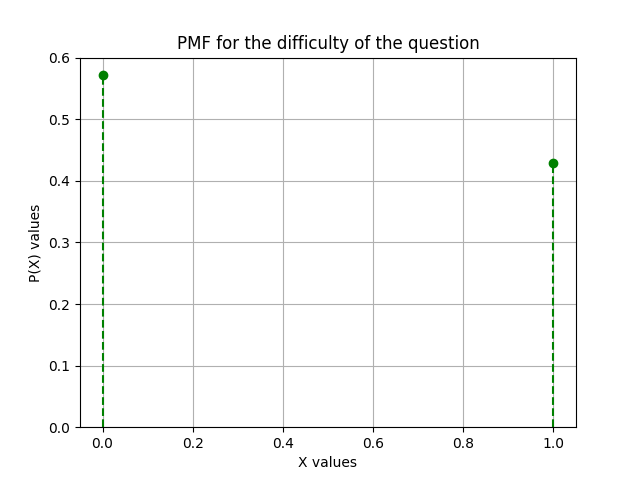
\includegraphics[width=\columnwidth]{pythonDifficultyPMF.png}
       \label{fig:Question Difficulty PMF}
       \caption{Question Difficulty P.M.F}
\end{figure}

\begin{figure}[!ht]
       \centering
       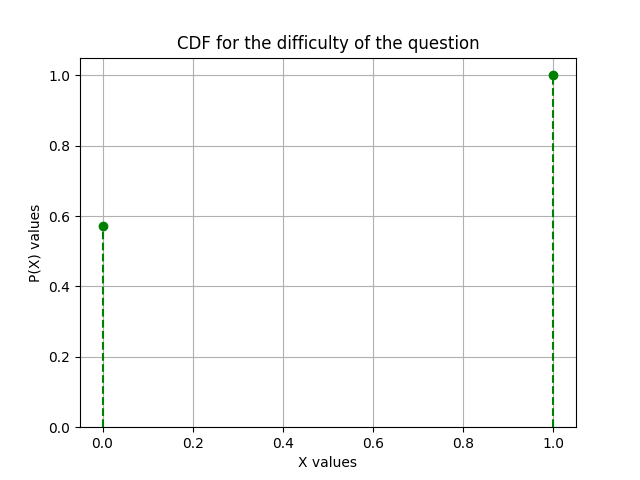
\includegraphics[width=\columnwidth]{pythonDifficultyCDF.png}
       \caption{Question Difficulty C.D.F}
       \label{fig:Question Difficulty CDF}
\end{figure}

\begin{figure}[!ht]
       \centering
       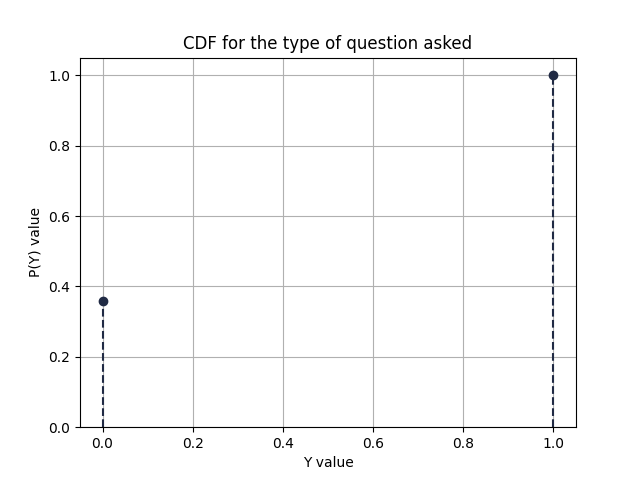
\includegraphics[width=\columnwidth]{pythonQuestionTypeCDF.png}
       \caption{Question Type C.D.F}
       \label{fig:Question Type CDF}
\end{figure}

\begin{figure}[!ht]
       \centering
       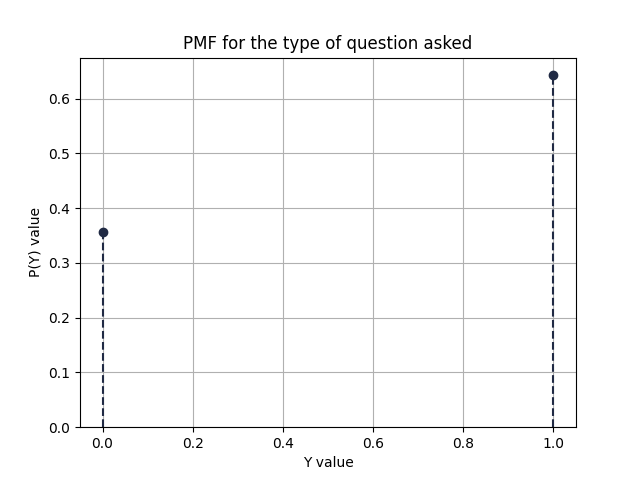
\includegraphics[width=\columnwidth]{pythonQuestionTypePMF.png}
       \caption{Question Type P.M.F}
       \label{fig:Question Type PMF}
\end{figure}

\end{document}